\section{Model Description}

The hinged rigid body class is an instantiation of the state effector abstract class. The state effector abstract class is a base class for modules that have dynamic states or degrees of freedom with respect to the rigid body hub. Examples of these would be reaction wheels, variable speed control moment gyroscopes, fuel slosh particles, etc. Since the state effectors are attached to the hub, the state effectors are directly affecting the hub as well as the hub is back affecting the state effectors.

Specifically, a hinged rigid body state effector is a rigid body that has a diagonal inertia with respect to its $\mathcal{S}_i$ frame as seen in Figure~\ref{fig:FlexFigure}. It is attached to the hub through a hinge with a linear torsional spring and linear damping term. The dynamics of this multi-body problem have been derived 

\begin{figure}[htbp]
	\centerline{
		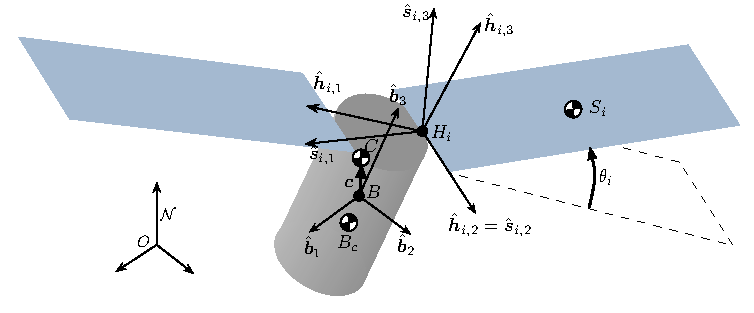
\includegraphics[width=0.8\textwidth]{Figures/Fig4_4_2}}
	\caption{Hinged rigid body frame and variable definitions}
	\label{fig:FlexFigure}
\end{figure}